\section{Concept Map}

Das Thema der vorliegenden Arbeit ist die Ausarbeitung des Algorithmus der Breitensuche in Form Lernprogrammartiger Unterlagen für das Gymnasium.  
Zu diesem Zweck wurde folgende Concept-Map (s. Abb.~\ref{fig:cmap}) entworfen, die sowohl das Vorwissen als auch einen kleinen Ausblick auf weitere Themen geben soll.
Dabei wurden solche Konzepte blau gefärbt, welche als Vorwissen schon bekannt sein sollten, aber im Rahmen dieser Arbeit nochmal wiederholt werden. 
Neue Konzepte wurden grün eingefärbt und werden in dieser Arbeit behandelt bzw. eingeführt werden sollen.
Weitere Konzepte, die nicht mehr in dieser Arbeit behandelt werden, wurden orange gefärbt. 

\begin{figure}[htb]
\begin{center}
%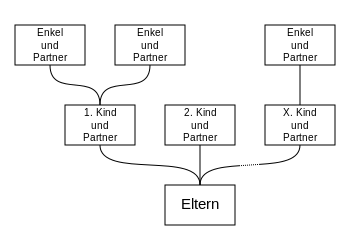
\includegraphics[width=.7\textwidth]{../fig/stammbaum.png}
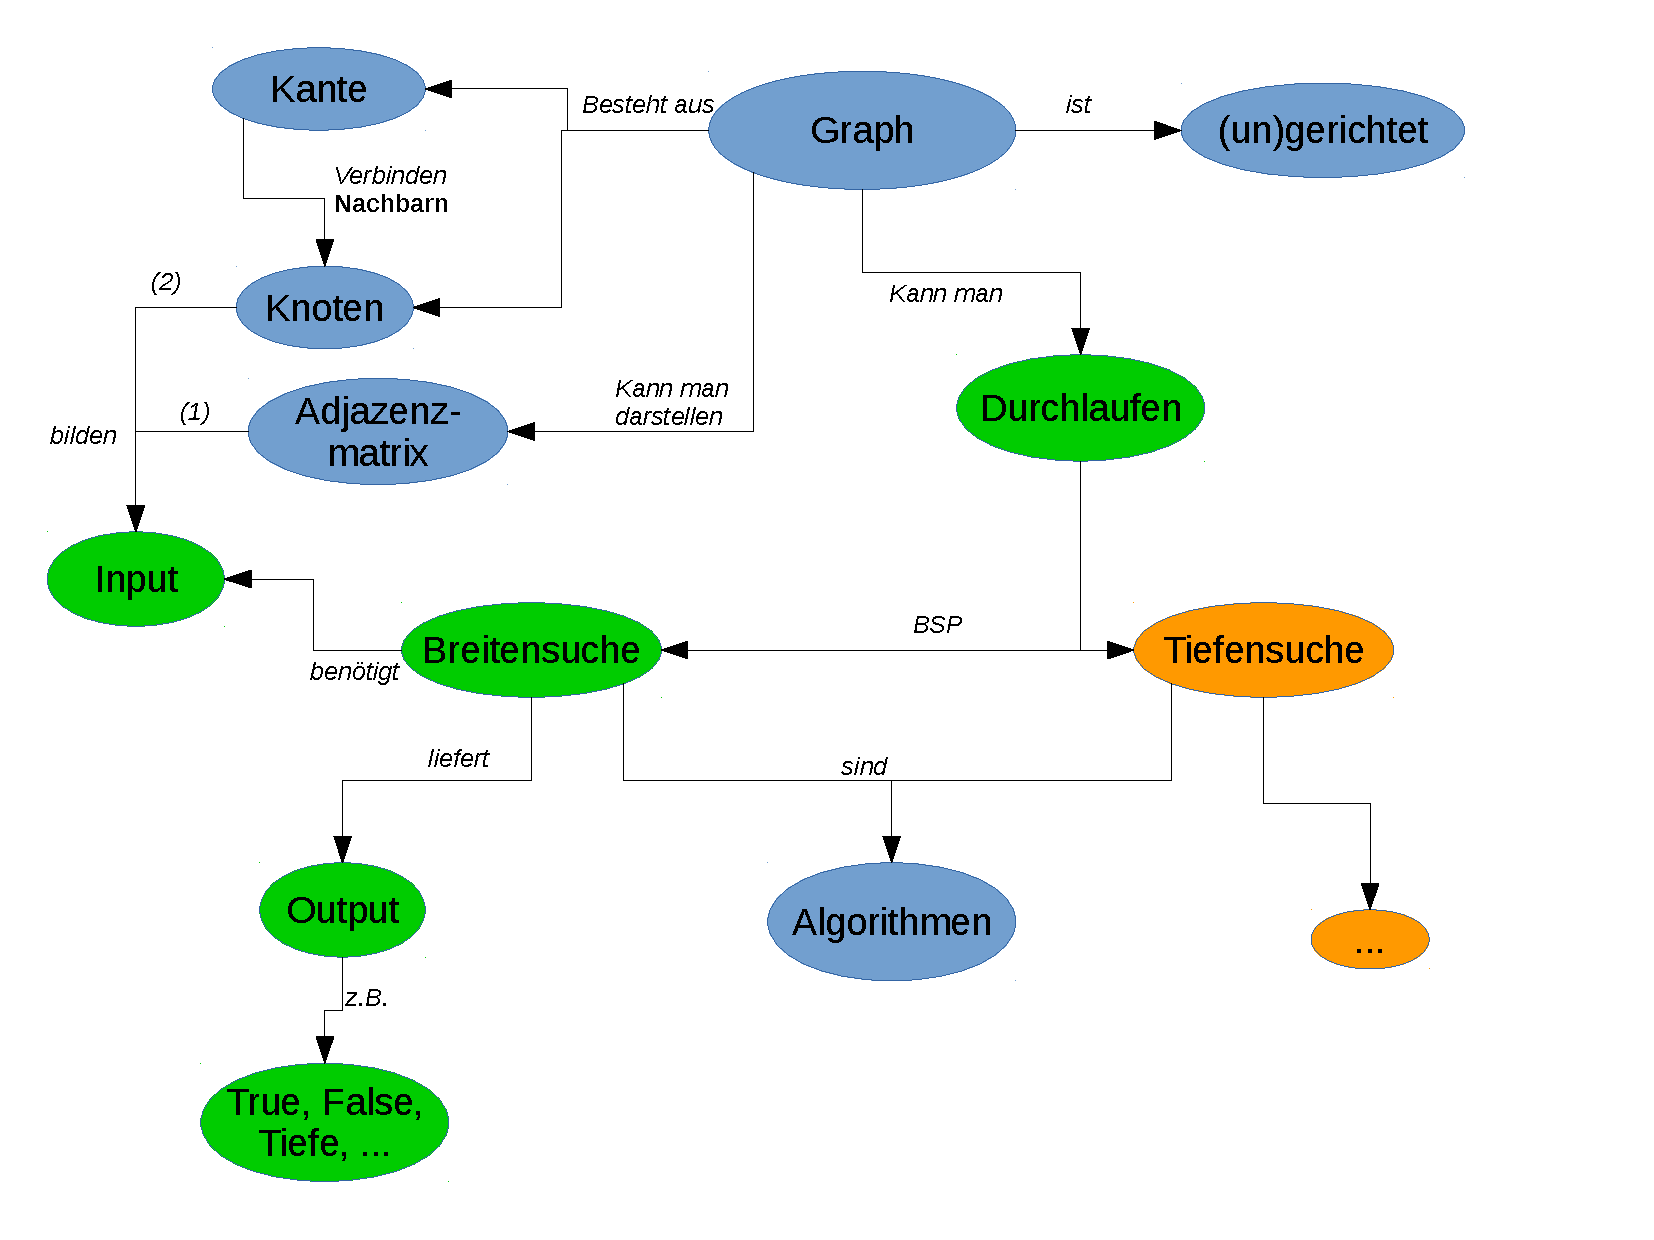
\includegraphics[width=.99\textwidth]{../cmap/bsuche_cmap.pdf}
\caption{Concept-Map zum Thema Breitensuche.
Blaue Konzepte und grüne Konzept werden in dieser Arbeit behandelt, wobei die Blauen das Vorwissen abbilden und Grüne neue Konzepte sind. 
Orangene Konzepte bilden einen Ausblick auf Konzepte, welche im Rahmen dieser Arbeit nicht mehr behandelt werden. 
}
\label{fig:cmap}
\end{center}
\end{figure}

Aus dieser Concept Map ergibt sich eine Sequenzierung des Unterrichts, bei dem zuerst die grundlegenden Begriffe eines Graphen repetiert werden, damit das Vorwissen der Sch\"uler aktiviert wird.

\section{Aufbau der LPU}

\subsection{F\"ur wen sind die LPU geeignet?}
Die Unterlagen richten sich an Sch\"ulerinnen und Sch\"uler der Gymnasialstufe und sind f\"ur den Informatikunterricht im Erg\"anzungsfach Informatik geeignet, idealerweise f\"ur Sch\"uler mit mathematisch/naturwissenschaftlichem Schwerpunkt. Es wird davon ausgegangen, dass die Sch\"uler bereits einige Grundlagen der Informatik kennengelernt haben, insbesondere den Begriff Algorithmus. Zum Vorwissen der Sch\"uler sollte ausserdem der Begriff des Graphen geh\"oren. Es wird davon ausgegangen, dass sie bereits einfache Programme in TigerJython schreiben k\"onnen und dabei wissen, wie Programme modular aufgebaut werden k\"onnen. Grundlegende Kenntnisse von elementaren Datentypen und Arrays sowie von Kontrollstrukturen werden f\"ur das L\"osen der Aufgaben vorausgesetzt. Es wird deshalb angenommen, dass die vorliegenden Unterlagen im zweiten Quartal des Erg\"anzungsfaches eingesetzt werden k\"onnen.

\subsection{Vorwissen}
Es wird davon ausgegangen, dass die Sch\"uler den Begriff des Graphen bereits kennen. Dieses Vorwissen soll zu Beginn nochmals aktiviert werden. Dabei werden die wichtigsten Begriffe repetiert: der Aufbau eines Graphen aus Knoten und Kanten, eines gerichteten oder ungerichteten Graphen sowie der Begriff von Nachbarsknoten. Damit wird eine klare Basis f\"ur die in den Unterlagen verwendeten Begriffe geschaffen.

Der Begriff des Algorithmus wird als Vorwissen vorausgesetzt, aber nicht nochmals aktiviert bzw. repetiert, da davon ausgegangen wird, dass sich die Sch\"uler schon vertiefter mit dem Begriff auseinandergesetzt haben und im Rahme des Erg\"anzungsfaches Informatik schon verschiedene Algorithmen kennengelernt bzw. entwickelt haben. Wir nehmen an, dass die Sch\"uler auch schon ein grundlegendes Verst\"andnis von Komplexit\"atsanalyse besitzen.

F\"ur die Implementationen und die Programmier\"ubungen werden keine Details repetiert, da die Sch\"uler auch hier im Rahmen des Erg\"anzungsfaches bereits einige Programme implementiert und die Grundlagen von Datentypen, Kontrollstrukturen und modularem Aufbaus kennengelernt und viel ge\"ubt haben. Wichtig sind f\"ur die Programmieraufgaben in diesen Unterlagen unter anderem Unterprogramme, Arrays und Schleifen.

Neue Begriffe und Konzepte werden in den Unterlagen so eingef\"uhrt, dass sie am vorhandenen Wissen ankn\"upfen und dieses erweitern.

\subsection{Konzeption}
Die Unterlagen sind so aufgebaut, dass schrittweise neue Konzepte eingef\"uhrt und erl\"autert werden. Im Fokus soll die Entwicklung beziehungsweise F\"orderung des Algorithmischen Denkens stehen. Die Sch\"uler sollen nicht nur das Konzept und die Anwendung der Breitensuche kennenlernen, sondern auch lernen, wie ein Algorithmus entwickelt wird und wie ein Algorithmus formuliert werden soll, damit er f\"ur eine breite Klasse von Problemen eingesetzt werden kann. Die LPU sollen dazu beitragen, dass die Sch\"uler sich intensiv mit der Formulierung der Problemstellung sowie der Entwicklung des Algorithmus auseinandersetzen und schlussendlich auch in der Lage sind, den Algorithmus zu implementieren.


\section{Lernziele}

Aus der Concept-Map lassen sich folgende Lernziele für diese Arbeit ableiten. 

\subsection{Leitidee}

Graphen spielen eine wichtige Rolle in unserem Alltag und werden sehr häufig zur Darstellung von Zusammenhängen verwendet (S-Bahnnetzwerk, Facebook, Websites, \dots). 
Mit diesen Netzwerken sind viele Fragen verbunden: Über wie viel Freundschaften bin ich mit einer anderen Person verbunden? Wie lange ist die kürzeste Verbindung von A nach B?
Damit man ein grundlegendes Verständnis dafür entwickelt, muss man sich überlegen, wie man sich auf Graphen bewegen kann. 
Eine Möglichkeit bietet die Breitensuche, welche einen naiven Einstieg bildet. 


\subsection{Dispositionsziel}

Die SuS wissen, dass man gewisse Probleme mit Hilfe von Graphen modellieren und mit Graphenalgorithmen lösen kann. 
Sie können Probleme analysieren und beurteilen, ob sie mit Hilfe von einer Breitensuche in einem Graphen gelöst werden können.



\subsection{Operationalisierte Lernziele}

Nach dieser Einheit können die SuS \dots

\begin{enumerate}
\item \dots die Begriffe und Unterschiede zur Darstellung von einfachen Graphen verstehen: (un)gerichtet, Knoten und Kante.

\item \dots verschiedene Darstellungsmöglichkeiten von Graphen aufzählen und diese ineinander überführen: Zeichnung, Knoten-/ Kantenmenge und Adjazenzmatrix.

\item \dots die Nachbarn von Knoten auf verschieden Darstellungen von Graphen bestimmen. 

\item \dots ein Programm schreiben, welches die Nachbarn eines Knoten eines bestimmten Knoten eines beliebigen Graphen ausgibt.


%%%TODO
%Breitensuche LZ so in Ordnung?


%\dots 
%Operationalisierte Lernziele:
%Die SuS können 
\item \dots die Funktionsweise einer Breitensuche in einem Graphen beschreiben.
%Die SuS können 
\item \dots für ein gegebenes Problem Breitensuche in einem Graphen anwenden.
%Die SuS können 
\item \dots ein gegebenes Problem mit einem Graphen modellieren und mittels Breitensuche eine Lösung finden.
% (evtl. spezifischer).
%Die SuS können 
\item \dots die Breitensuche in Tiger Jython implementieren.
%Die SuS können 
\item \dots die Laufzeit einer Breitensuche beurteilen.
% (sofern O notation bekannt…)
%Die SuS können 
\item \dots den Speicherbedarf der Breitensuche beurteilen.


\end{enumerate}

\section{Inhalt}

Aus der Concept-Map und den Lernzielen ergibt sich folgender Ablauf für die LPU:
In einem ersten Abschnitt werden nochmal die Grundlagen zu Graphen und ihrer Darstellungen wiederholt und anhand von Beispielen und Aufgaben geübt. 
Dabei wird darauf geachtet zuerst eine zeichnerische Darstellung, dann eine Mengendarstellung und zum Schluss die Adjazenzmatrix einzuführen. 
Hierbei wurde sich an \cite{cormen,ottmann} orientiert.
Zum Schluss des ersten Abschnitts soll mit der Einführung von Nachbarn und dem Schreiben eines solchen Programms eine Vorarbeit für den kommenden Abschnitt gelegt werden.

Im zweiten Abschnitt werden Grundlagen \"uber das Modellieren von Problemen mit Hilfe von Graphen und das L\"osen der Probleme mit Hilfe von Graphenalgorithmen vermittelt. Insbesondere werden Problemstellungen betrachtet, die sich mit Hilfe von der Breitensuche l\"osen lassen. Der Algorithmus f\"ur die Breitensuche wird Schritt f\"ur Schritt erarbeitet, erweitert und implementiert sowie an konkreten Beispielen angewendet. F\"ur den Algorithmus wird ein Vorgehen mit F\"arben von Knoten verwendet, wie es auch in \cite{cormen} zu finden ist.